\documentclass[10pt,twocolumn]{article}

\usepackage[letterpaper,margin=0.68in]{geometry}
\usepackage{graphicx}
\usepackage{booktabs}
\usepackage{array}
\usepackage{caption}
\usepackage{hyperref}
\usepackage{xcolor}
\usepackage{enumitem}
\usepackage{placeins}

\captionsetup{font=small,labelfont=bf}
\setlist[itemize]{leftmargin=*,nosep}
\setlength{\columnsep}{0.22in}
\setlength{\textfloatsep}{8pt plus 2pt minus 2pt}
\setlength{\floatsep}{8pt plus 2pt minus 2pt}
\setlength{\intextsep}{8pt plus 2pt minus 2pt}
\raggedbottom

\title{\vspace{-0.4in}Field Agave Detection and Line-Crossing Count from RGB Video Using YOLO26}
\author{Raul Venegas \\ Local thesis repository: \texttt{deteccion de agave}}
\date{}

\begin{document}
\maketitle

\begin{abstract}
Early-stage agave fields require timely plant localization before selective weed-control actuation can be attempted. This paper reports a reproducible computer-vision stage for agave detection and operational line-crossing count from RGB field imagery. A Roboflow project was verified live as \texttt{raul-stlme/agave-vty65}, with 404 images, a single \texttt{agave} class, and train/validation/test splits of 295/73/36 images. The local export used for training contains 4,371 YOLO boxes and all images are 2880 by 1620 pixels. Eleven YOLO26 experiments were compared; the best run, \texttt{yolo26s\_sgd\_cos\_slow\_120e}, reached 0.693 precision, 0.615 recall, 0.654 mAP50, and 0.213 mAP50-95 on the test split. Sanity checks found all labels in bounds, one class only, uniform image dimensions, and no duplicate-box pairs above IoU 0.80. A BoT-SORT-style tracking test on a 30 s video segment counted 41 unique downward line crossings. The study is intentionally scoped as an agave-detection baseline: weed detection, metric plant dimensions, and embedded actuation remain future work.
\end{abstract}

\section{Introduction}

The thesis project targets machine vision for precision management in young agave rows, where weed competition can affect crop establishment and where manual or blanket control strategies are costly. The present stage does not yet solve weed recognition. Instead, it establishes the crop-detection component needed before selective weeding can be made spatially reliable: agaves must be detected in cluttered RGB field scenes and then followed in video well enough to produce operational counts.

Deep learning has become a central method in agricultural vision because it can learn field-specific appearance variation from images rather than relying on hand-crafted color or texture rules \cite{kamilaris2018}. Weed recognition remains difficult because crop and weed plants can share color, texture, and early growth-stage structure \cite{hasan2021}. For this reason, this work reports a narrower and auditable milestone: single-class agave detection, model selection across local experiments, and a video tracking/counting proof of workflow.

The contribution is practical. First, the data source was verified against Roboflow live rather than inferred only from local files. Second, the local export actually used for training was audited for split balance, bounding-box geometry, label validity, possible duplicate boxes, and version drift. Third, the best YOLO26 run was selected from a benchmark of 11 experiments and connected to a reproducible line-crossing count.

\section{Related Work}

YOLO-family detectors are designed for real-time object detection, making them attractive for field robotics where latency and deployment simplicity matter. The current repository uses YOLO26 weights; Jocher et al. describe YOLO26 as a real-time model family with deployment-oriented detection heads and scale variants \cite{jocher2026}. The evaluation follows object-detection metrics commonly used for bounding-box detectors, including precision, recall, mAP50, and mAP50-95; Padilla et al. review how object-detection metrics and annotation formats affect interpretation \cite{padilla2021}.

The video component follows the tracking-by-detection pattern: detections are produced per frame and then associated over time. SORT established a simple online association baseline using Kalman filtering and Hungarian matching, while later trackers such as ByteTrack showed that retaining lower-confidence detections during association can reduce fragmented trajectories \cite{bewley2016,zhang2022}. In this repository, the operational tracker is configured through a BoT-SORT YAML file in the Ultralytics workflow; the paper therefore treats tracking as a deployment test rather than a new tracking algorithm.

\section{Materials and Methods}

\subsection{Live Source Verification}

The local dataset metadata originally pointed to \texttt{raul-stlme/raul-stlme}. A live Roboflow workspace query showed that the actual project ID is \texttt{raul-stlme/agave-vty65}, project name \texttt{agave}. The live project reports 404 images, split as 295 training, 73 validation, and 36 test images, and a single \texttt{agave} class. A live image search returned the same 404 images and the same split counts.

Two versioning warnings were kept in the evidence rather than hidden. First, the project summary reports 4,374 \texttt{agave} annotations, the live image-by-image search sums 4,373, and the local export used by the benchmark contains 4,371 boxes. The difference is localized to one image, where the local export has 9 boxes and Roboflow live has 11. Second, Roboflow version 1 reports 699 generated images with resizing/augmentation; this is not the local 404-image export used for the benchmark. Therefore, all model-performance results below are tied to the local export, while Roboflow live is used to verify source identity, splits, class vocabulary, and version drift.

\subsection{Dataset Audit}

The local dataset contains 404 RGB images, all 2880 by 1620 pixels, and 4,371 YOLO boxes. Table \ref{tab:dataset} summarizes the split-level counts. Bounding-box distributions, complete percentiles, and coefficient of variation are stored in \texttt{evidencia/estadisticas\_agave\_tesis.json}.

\begin{table}[t]
\centering
\caption{Local export used for training and evaluation.}
\label{tab:dataset}
\begin{tabular}{lrrrr}
\toprule
Split & Images & Boxes & Mean boxes/img & P95 \\
\midrule
Train & 295 & 3175 & 10.76 & 18.0 \\
Val & 73 & 793 & 10.86 & 19.4 \\
Test & 36 & 403 & 11.19 & 17.0 \\
\midrule
Total & 404 & 4371 & 10.82 & 18.0 \\
\bottomrule
\end{tabular}
\end{table}

Sanity checks were applied before interpreting model results. All labels remained inside normalized YOLO bounds, all labels used the expected single class ID, all images had the same 16:9 resolution, and the local export contained no 640 by 640 files. Pairwise same-image duplicate screening found 0 box pairs above IoU 0.90 and 0 above IoU 0.80. Because no calibrated camera model or ground sampling distance was available, the analysis does not infer plant diameter, area, or real-world spacing.

\begin{figure*}[t]
\centering
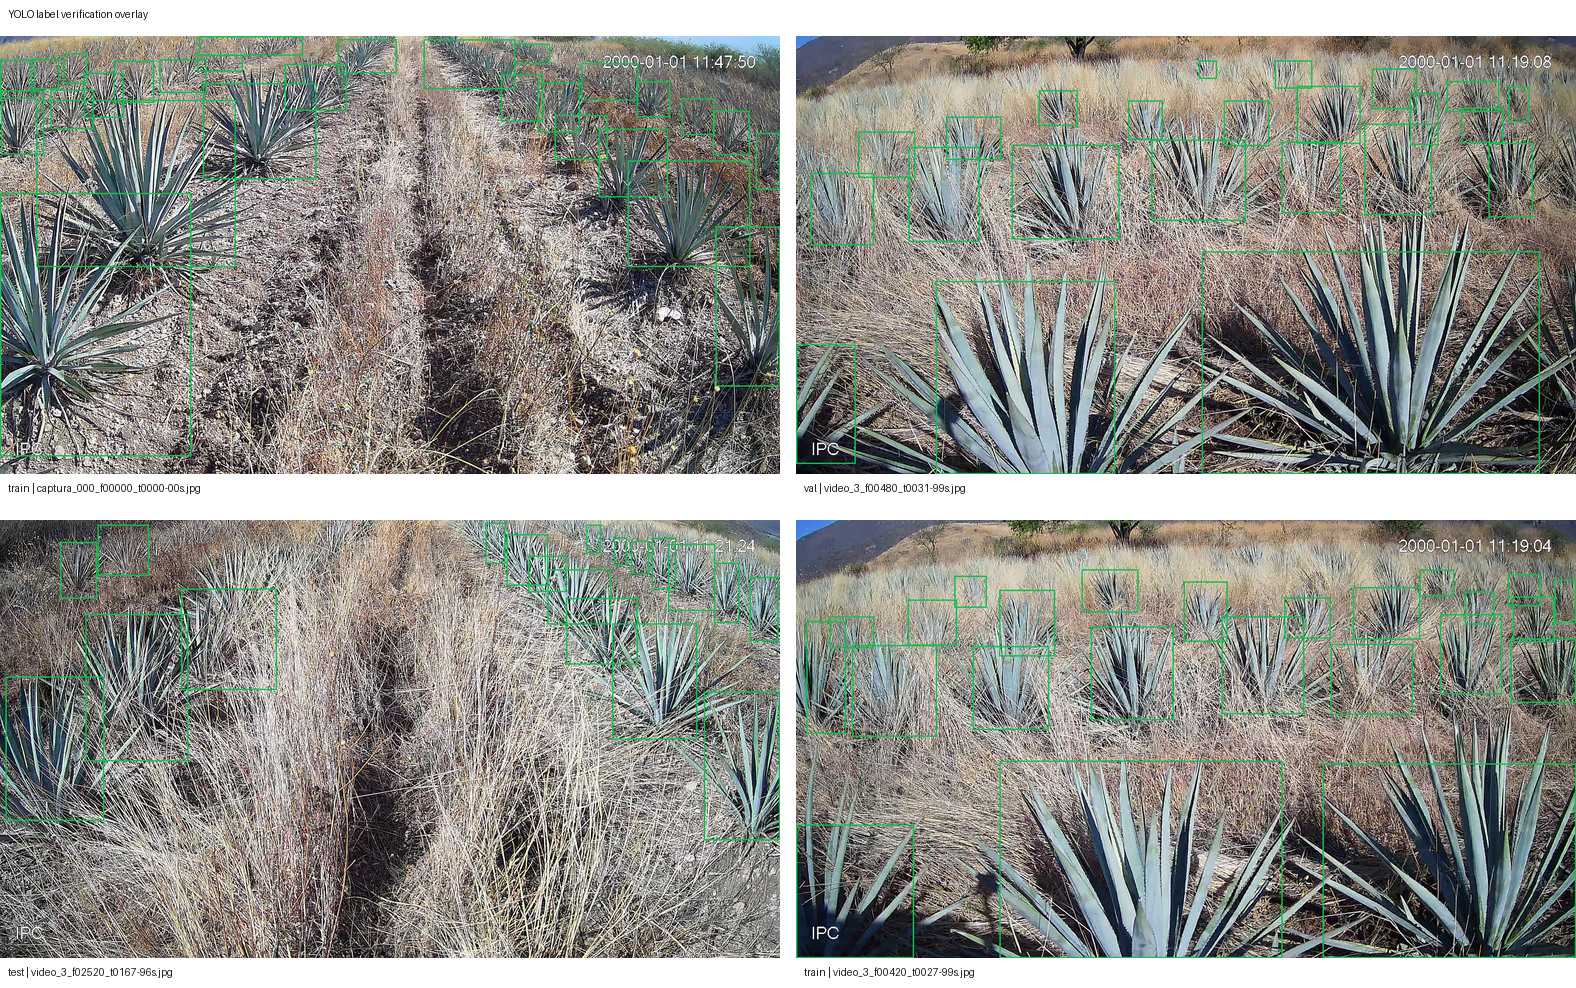
\includegraphics[width=0.96\textwidth]{../evidencia/figuras_en/fig01_overlay_verificacion_agave.png}
\caption{Verification overlay from the local YOLO labels. The panels show representative training, validation, and test images with agave boxes drawn directly from the local export used by the benchmark.}
\label{fig:overlay}
\end{figure*}

\subsection{Training and Model Selection}

The best local run was \texttt{yolo26s\_sgd\_cos\_slow\_120e}. It used \texttt{yolo26s.pt}, image size 640 during training, batch size 8, SGD with initial learning rate 0.005, cosine learning-rate scheduling, 120 configured epochs, and early stopping with patience 30. The run recorded 86 epochs; the best validation mAP50-95 epoch was 56.

Eleven runs were compared using the repository benchmark CSV. The four primary test metrics were precision, recall, mAP50, and mAP50-95. Across all runs, mean test precision was 0.6075, mean recall was 0.5408, mean mAP50 was 0.5691, and mean mAP50-95 was 0.1838. The winning run improved all four metrics relative to these means.

\subsection{Video Tracking and Count}

The selected model was applied to a 30 s field-video segment corresponding to 01:30--02:00 of \texttt{3.mp4}. The tracking command used the local BoT-SORT configuration, \texttt{conf=0.30}, \texttt{iou=0.40}, \texttt{imgsz=640}, a horizontal line at 50\% of the frame, downward direction, and unique-ID counting. The resulting CSV is the line-crossing file in \texttt{video\_predictions/}.

\section{Results}

\subsection{Dataset Geometry and Label Quality}

The dataset is moderately dense for a single-class field detector: the median image has 11 boxes and the 95th percentile has 18 boxes. The normalized bounding-box width has mean 0.0860 and P95 0.1729; normalized height has mean 0.1782 and P95 0.4272. The larger height than width is consistent with upright agave plants seen from an oblique ground-level perspective. The normalized box-area distribution is highly variable (CV 1.161), confirming that the detector must handle both small distant plants and larger foreground plants.

\begin{figure}[t]
\centering
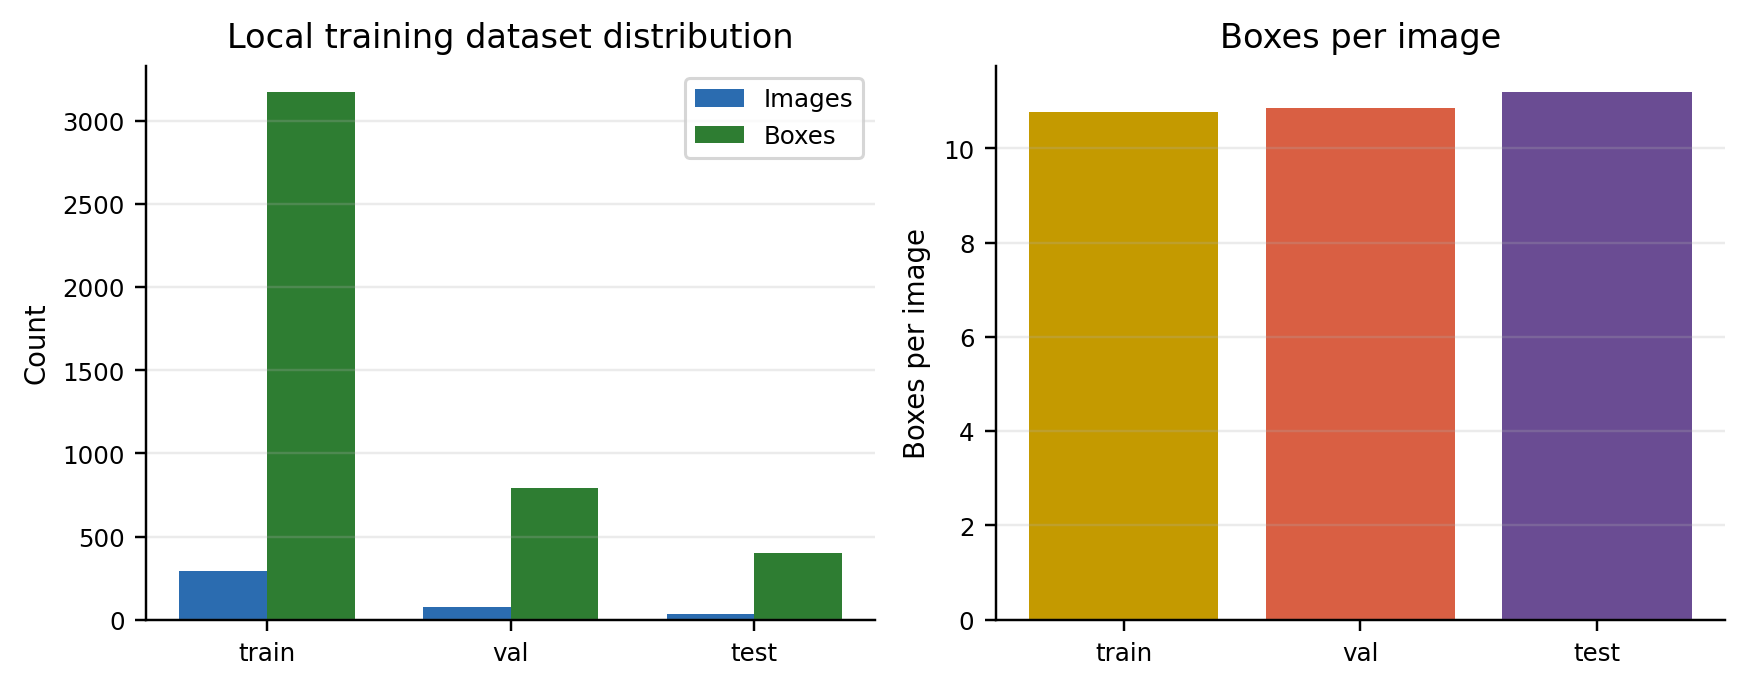
\includegraphics[width=\columnwidth]{../evidencia/figuras_en/fig02_distribucion_dataset.png}
\caption{Image and annotation distribution by split. Box density is similar across train, validation, and test splits.}
\label{fig:dataset}
\end{figure}

\begin{figure}[t]
\centering
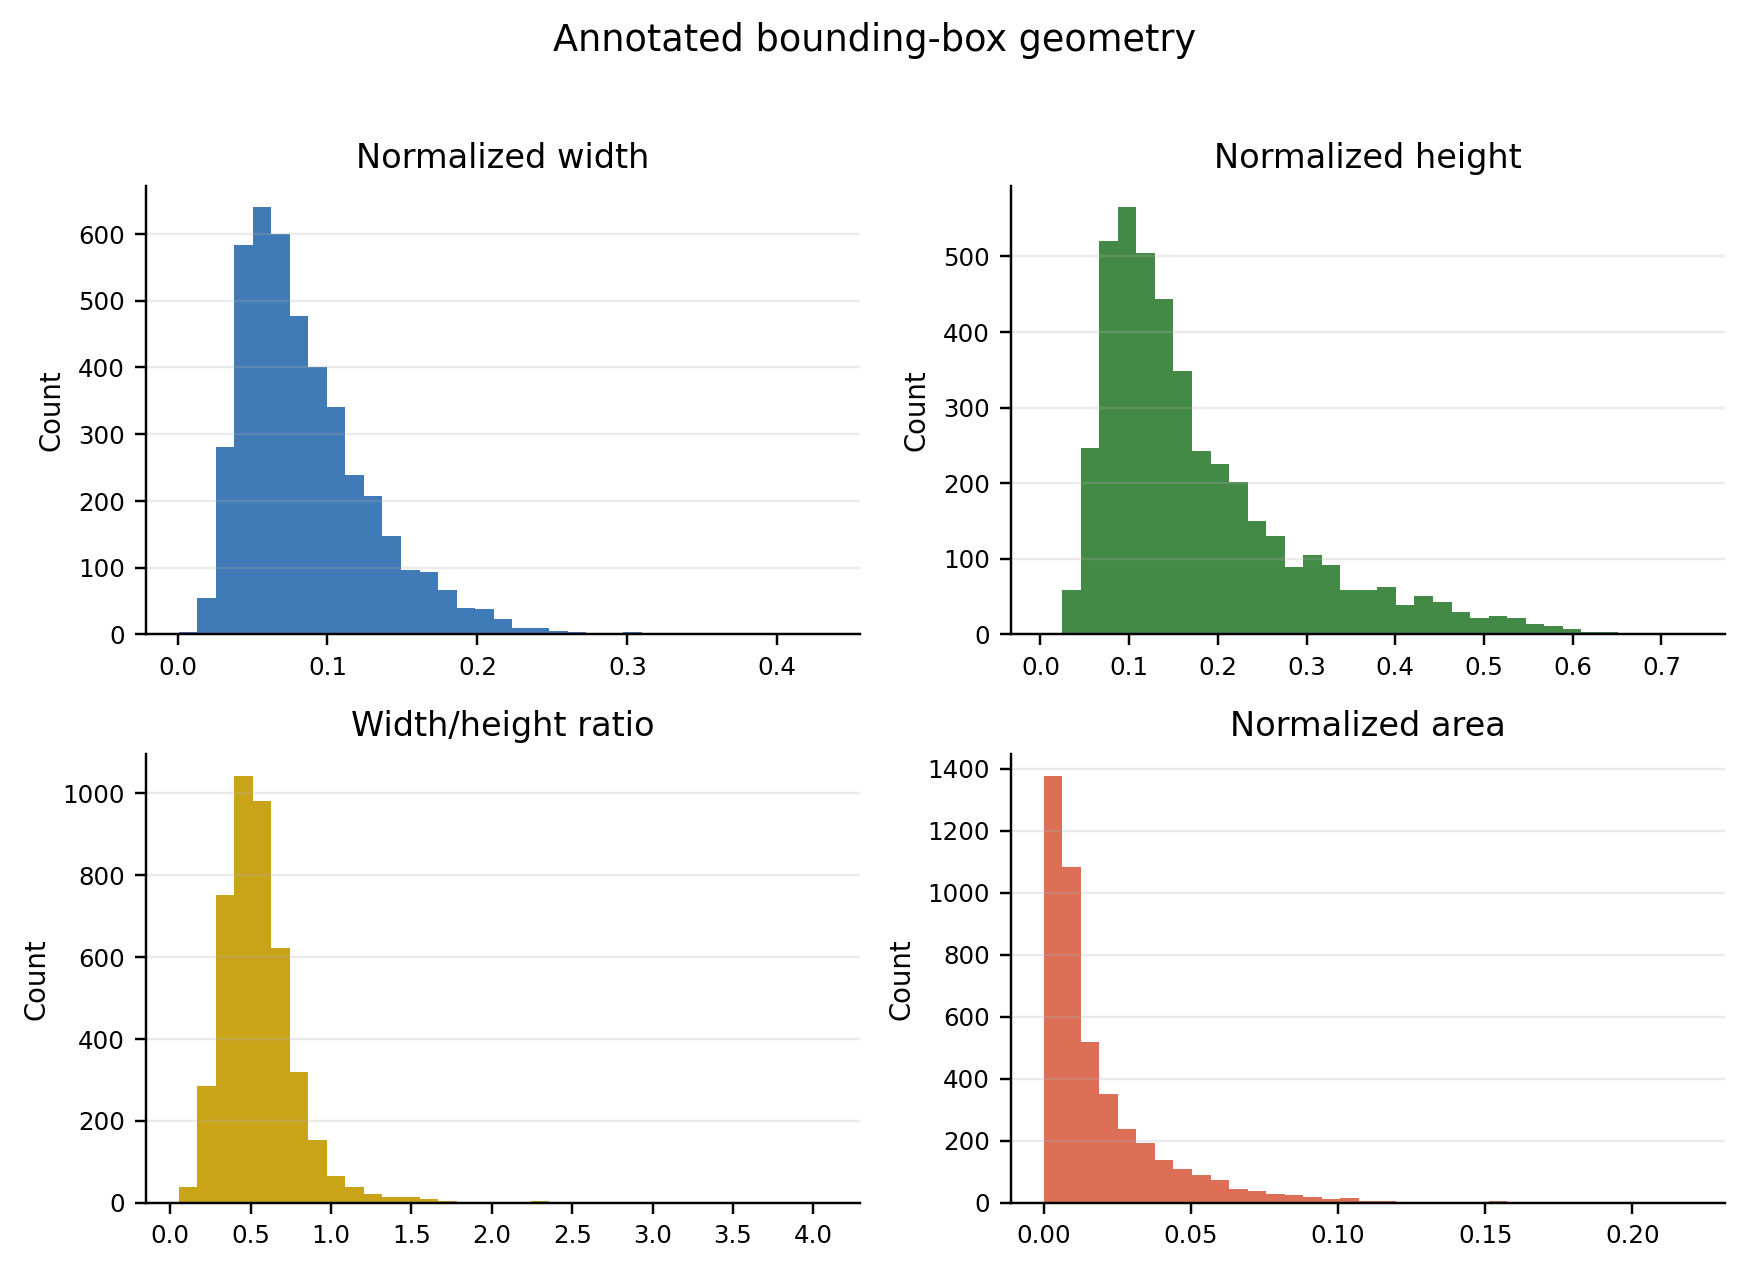
\includegraphics[width=\columnwidth]{../evidencia/figuras_en/fig03_geometria_bboxes.png}
\caption{Bounding-box geometry in the local export. The broad area distribution reflects strong scale variation in the field imagery.}
\label{fig:bbox}
\end{figure}

\subsection{Benchmark Performance}

The best model reached 0.693 precision, 0.615 recall, 0.654 mAP50, and 0.213 mAP50-95 on the test split. The generated benchmark chart in \texttt{evidencia/figuras\_en/} shows that the winning run ranks first in both mAP50 and mAP50-95, although several experiments cluster near mAP50 of 0.59--0.61. Figure \ref{fig:training} shows fast early metric gains followed by noisy but stable validation performance. The gap between mAP50 and mAP50-95 is the most important caution: the model often localizes plants well enough at IoU 0.50, but stricter overlap thresholds still expose localization error. For mechanical actuation, that matters more than it would for a visual-only inventory.

\begin{figure*}[t]
\centering
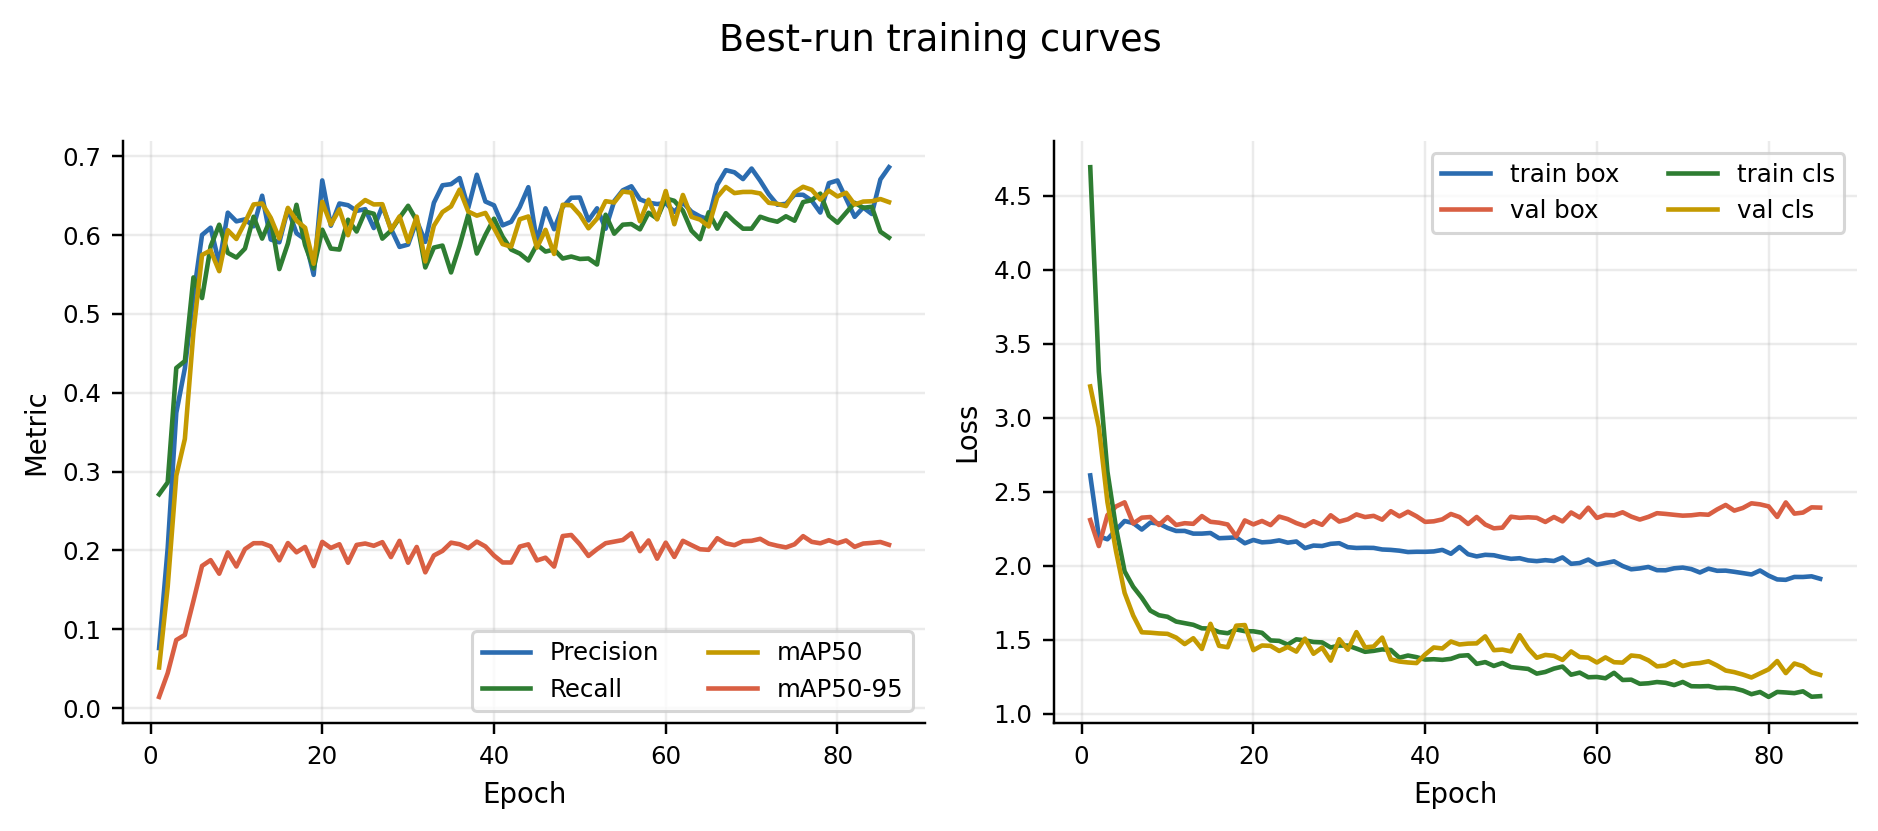
\includegraphics[width=0.88\textwidth]{../evidencia/figuras_en/fig06_curvas_entrenamiento_mejor_modelo.png}
\caption{Training curves for the selected run. The best epoch by validation mAP50-95 is epoch 56, while training continued to epoch 86 before stopping.}
\label{fig:training}
\end{figure*}

\subsection{Operational Count}

The tracking CSV contains 41 events and 41 unique track IDs, all counted in the downward direction. The first counted crossing occurs at 0.400 s and the last at 29.994 s. Figure \ref{fig:tracking} shows the final frame and cumulative count. This supports the workflow from detection to tracking to a usable line-crossing count, but it is not a formal count-accuracy evaluation because no independent manual ground truth for every crossing is included.

\begin{figure*}[t]
\centering
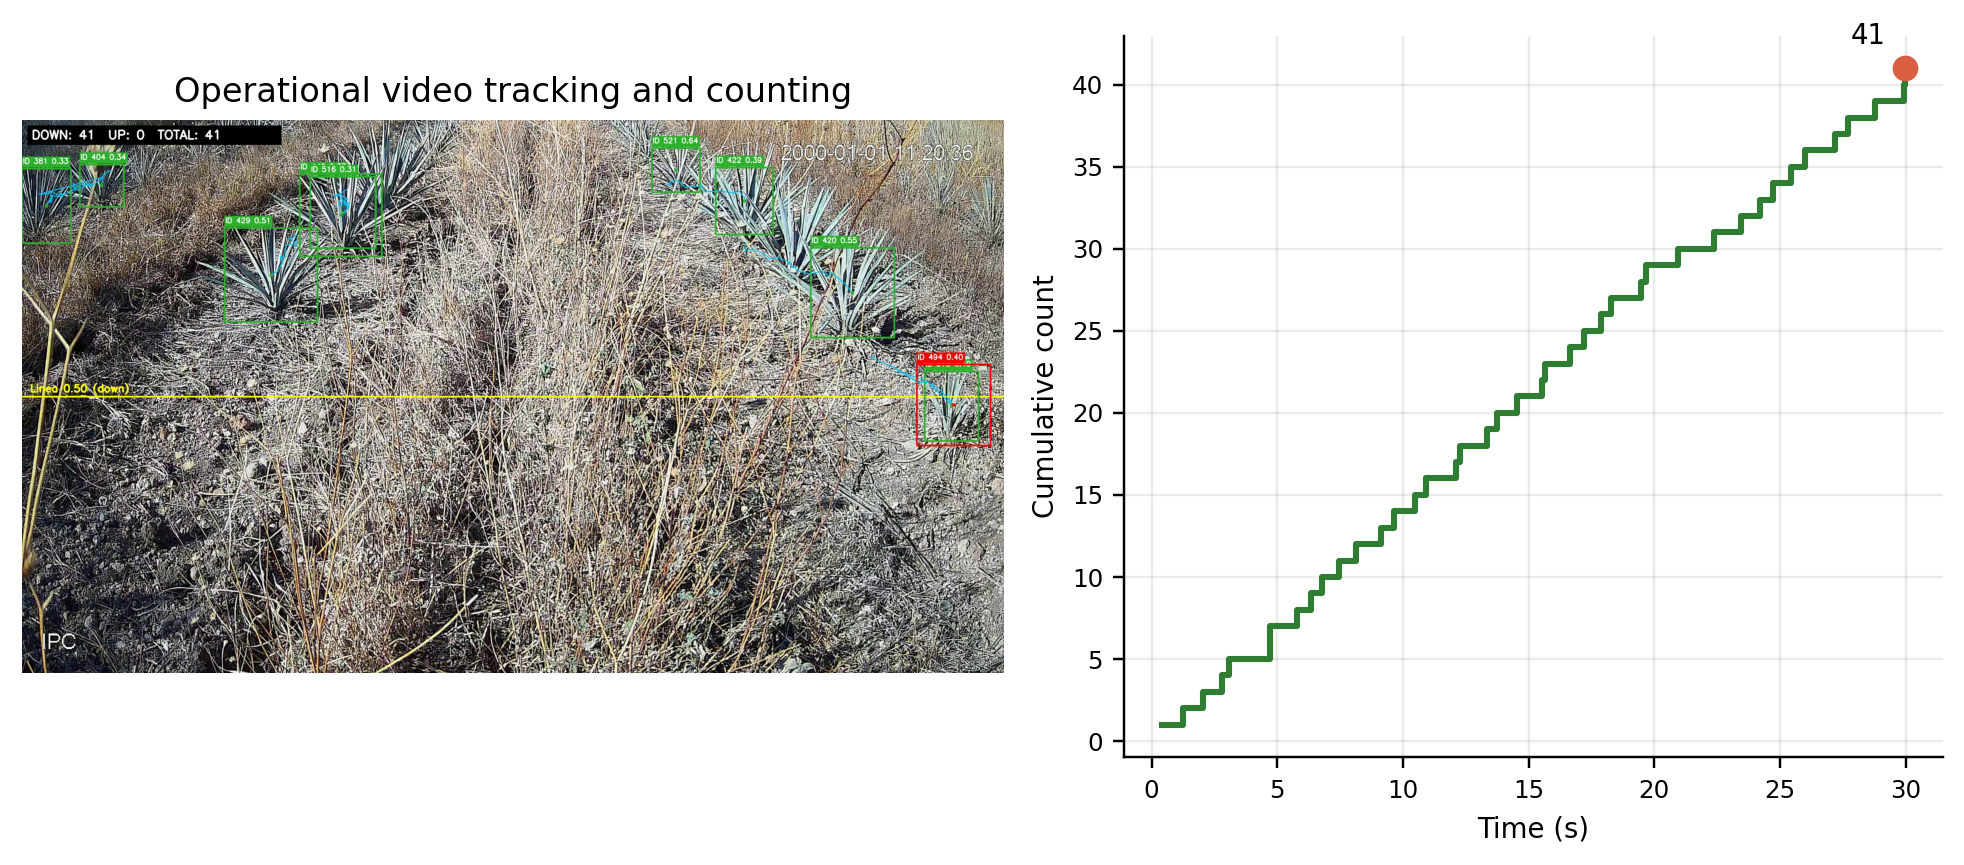
\includegraphics[width=0.94\textwidth]{../evidencia/figuras_en/fig08_tracking_conteo.png}
\caption{Operational tracking evidence. The final annotated frame reports 41 downward crossings, and the cumulative curve reproduces the count from the CSV.}
\label{fig:tracking}
\end{figure*}

\subsection{Versioning Evidence}

The generated versioning figure in \texttt{evidencia/figuras\_en/} summarizes why the local export is treated as the experimental dataset. Roboflow live confirms the same 404 source images and splits, but its aggregate annotation counts differ slightly from the local export, and its generated version contains 699 images. The paper therefore avoids mixing Roboflow version-1 model metadata with the local benchmark.

\FloatBarrier

\section{Discussion}

The evidence supports three findings. First, the data export is usable for single-class agave detection: labels are bounded, duplicate-box screening found no high-IoU duplicates, and box density is comparable across splits. Second, YOLO26s with SGD and cosine scheduling is the strongest tested configuration in this repository, but the mAP50-95 value of 0.213 shows that localization precision is still limited. Third, the tracking/counting stage demonstrates a working operational chain over video, producing 41 unique downward crossings.

The results also define the next experimental priorities. More data should be added for the weed class before the thesis can claim crop/weed discrimination. A manually verified line-crossing ground truth is needed to convert the operational count into a count-accuracy result. Finally, camera calibration or a measured field scale is required before bounding boxes can support physical plant dimensions or actuator-offset distances. Without that calibration, image-space detections are useful for visual tracking but not yet for metric actuation.

\section{Conclusions}

A reproducible agave-detection baseline was built from the local thesis repository. The live Roboflow project was verified, the local 404-image export was audited, and the best of 11 YOLO26 experiments reached 0.654 mAP50 and 0.213 mAP50-95 on the test split. Label sanity checks passed, no duplicate boxes above IoU 0.80 were found, and a 30 s video segment produced a 41-agave unique line-crossing count. The paper should be read as a validated crop-detection and counting milestone. Its main limitations are the single-class dataset, the small test split, the lack of manual count ground truth, and the absence of GSD/camera calibration.

\section*{Reproducibility}

All numbers in this paper are generated from \texttt{evidencia/estadisticas\_agave\_tesis.json}. The figures are generated with the repository \texttt{.venv} Python by:

\begin{verbatim}
src\analisis_extendido.py
  --env-file <path-to-env>
src\analisis_agave_tesis.py --lang es
src\figuras_en.py
\end{verbatim}

The scripts intentionally do not store API keys. The local evidence files are under \texttt{evidencia/}; paper inputs are under \texttt{paper/}.

{\small
\begin{thebibliography}{6}

\bibitem{jocher2026}
G. Jocher, J. Qiu, M. Liu, S. Lyu, F. C. Akyon, and M. E. Kalfaoglu, ``Ultralytics YOLO26: Unified Real-Time End-to-End Vision Models,'' arXiv:2606.03748, 2026. doi: \href{https://doi.org/10.48550/arXiv.2606.03748}{10.48550/arXiv.2606.03748}.

\bibitem{padilla2021}
R. Padilla, W. L. Passos, T. L. B. Dias, S. L. Netto, and E. A. B. da Silva, ``A Comparative Analysis of Object Detection Metrics with a Companion Open-Source Toolkit,'' \textit{Electronics}, vol. 10, no. 3, p. 279, 2021. doi: \href{https://doi.org/10.3390/electronics10030279}{10.3390/electronics10030279}.

\bibitem{bewley2016}
A. Bewley, Z. Ge, L. Ott, F. Ramos, and B. Upcroft, ``Simple Online and Realtime Tracking,'' in \textit{2016 IEEE International Conference on Image Processing (ICIP)}, 2016, pp. 3464--3468. doi: \href{https://doi.org/10.1109/ICIP.2016.7533003}{10.1109/ICIP.2016.7533003}.

\bibitem{zhang2022}
Y. Zhang, P. Sun, Y. Jiang, D. Yu, F. Weng, Z. Yuan, P. Luo, W. Liu, and X. Wang, ``ByteTrack: Multi-object Tracking by Associating Every Detection Box,'' in \textit{Computer Vision -- ECCV 2022}, Lecture Notes in Computer Science, vol. 13682, Springer, 2022, pp. 1--21. doi: \href{https://doi.org/10.1007/978-3-031-20047-2_1}{10.1007/978-3-031-20047-2\_1}.

\bibitem{kamilaris2018}
A. Kamilaris and F. X. Prenafeta-Boldu, ``Deep learning in agriculture: A survey,'' \textit{Computers and Electronics in Agriculture}, vol. 147, pp. 70--90, 2018. doi: \href{https://doi.org/10.1016/j.compag.2018.02.016}{10.1016/j.compag.2018.02.016}.

\bibitem{hasan2021}
A. S. M. M. Hasan, F. Sohel, D. Diepeveen, H. Laga, and M. G. K. Jones, ``A survey of deep learning techniques for weed detection from images,'' \textit{Computers and Electronics in Agriculture}, vol. 184, article 106067, 2021. doi: \href{https://doi.org/10.1016/j.compag.2021.106067}{10.1016/j.compag.2021.106067}.

\end{thebibliography}
}

\end{document}
